\documentclass[12pt]{article}

% MLA format
\usepackage[letterpaper]{geometry}
\usepackage{times}
\geometry{top=1.0in, bottom=1.0in, left=1.0in, right=1.0in}
\usepackage{fancyhdr}
\pagestyle{fancy}
\lhead{} 
\chead{} 
\rhead{Simmons \thepage} 
\lfoot{} 
\cfoot{} 
\rfoot{}
\renewcommand{\headrulewidth}{0pt} 
\renewcommand{\footrulewidth}{0pt} 

\usepackage{mdwlist}
\usepackage{enumitem}
\setlist{  
  listparindent=\parindent,
  parsep=0pt,
}
\title{Homework 5}
\author{Mark Simmons}
\date{February 28, 2020}

% Multi-line glosses
%\usepackage{chngcntr}
%\usepackage{gb4e,cgloss4e}

%\newcounter{glossnum}

%\newcommand{\numgloss}{\refstepcounter{glossnum}\alph{glossnum}.\space}
%\counterwithin{glossnum}{xnumi}
%\renewcommand{\theglossnum}{\thexnumi\alph{glossnum}}

% Typing in IPA
\usepackage{tipa}

% Sentence trees
\usepackage{tikz-qtree}
\usepackage{lscape}
\usepackage{graphicx}
\tikzset{level distance=30pt,
    sibling distance=6pt,
    every tree node/.style={align=center},
    }

\begin{document}

\maketitle

\begin{enumerate}

% question 1
\item Domination
\begin{enumerate}[label=\arabic*)]
\item D$_{1}$ is dominated by \underline{NP$_{1}$}, TP$_{1}$
\item D$_{2}$ is dominated by \underline{NP$_{2}$}, TP$_{2}$, CP, VP$_{1}$, TP$_{1}$
\item N$_{1}$ is dominated by \underline{NP$_{1}$}, TP$_{1}$
\item N$_{2}$ is dominated by \underline{NP$_{2}$}, TP$_{2}$, CP, VP$_{1}$, TP$_{1}$
\item V$_{1}$ is dominated by \underline{VP$_{1}$}, TP$_{1}$
\item V$_{2}$ is dominated by \underline{VP$_{2}$}, TP$_{2}$, CP, VP$_{1}$, TP$_{1}$
\item Adv is dominated by \underline{AdvP}, VP$_{2}$, TP$_{2}$, CP, VP$_{1}$, TP$_{1}$
\item C is dominated by \underline{CP}, VP$_{1}$, TP$_{1}$
\item No nodes dominate TP$_{1}$
\item TP$_{2}$ is dominated by \underline{CP}, VP$_{1}$, TP$_{1}$
\item NP$_{1}$ is dominated by \underline{TP$_{1}$}
\item NP$_{2}$ is dominated by \underline{TP$_{2}$}, CP, VP$_{1}$, TP$_{1}$
\item VP$_{1}$ is dominated by \underline{TP$_{1}$}
\item VP$_{2}$ is dominated by \underline{TP$_{2}$}, CP, VP$_{1}$, TP$_{1}$
\item CP is dominated by \underline{VP$_{1}$}, TP$_{1}$
\item AdvP is dominated by \underline{VP$_{2}$}, TP$_{2}$, CP, VP$_{1}$, TP$_{1}$
\item The root node is TP$_{1}$
\item The terminal nodes are D$_{1}$ \emph{the}, N$_{1}$ \emph{baker}, V$_{1}$ \emph{said}, C \emph{that}, D$_{2}$ \emph{his}, N$_{2}$ \emph{bread}, V$_{2}$ \emph{smelled}, Adv \emph{glorious}\
\item The non-terminal nodes are TP$_{1}$, NP$_{1}$, VP$_{1}$, CP, TP$_{2}$, NP$_{2}$, VP$_{2}$, AdvP
\item VP$_{2}$ dominates V$_{2}$, AdvP, and Adv
\item CP dominates C, TP$_{2}$, NP$_{2}$, D$_{2}$, N$_{2}$, VP$_{2}$, V$_{2}$, AdvP and Adv
\item NP$_{1}$ dominates D$_{1}$ and N$_{1}$
\end{enumerate}

% question 2
\item C-command
\begin{enumerate}[label=\arabic*)]
\item D$_{1}$ c-commands \underline{N$_{1}$}
\item D$_{2}$ c-commands \underline{N$_{2}$}
\item N$_{1}$ c-commands \underline{D$_{1}$}
\item N$_{2}$ c-commands \underline{D$_{2}$}
\item V$_{1}$ c-commands \underline{CP}, C, TP$_{2}$, NP$_{2}$, VP$_{2}$, D$_{2}$, N$_{2}$, V$_{2}$, AdvP, Adv
\item V$_{2}$ c-commands \underline{AdvP}, Adv
\item Adv does not c-command any node
\item C c-commands \underline{TP$_{2}$}, NP$_{2}$, VP$_{2}$, D$_{2}$, N$_{2}$, V$_{2}$, AdvP, Adv
\item TP$_{1}$ does not c-command any node
\item TP$_{2}$ c-commands \underline{C}
\item NP$_{1}$ c-commands \underline{VP$_{1}$}, V, CP, C, TP$_{2}$, NP$_{2}$, VP$_{2}$, D$_{2}$, N$_{2}$, V$_{2}$, AdvP, Adv
\item NP$_{2}$ c-commands \underline{VP$_{2}$}, V$_{2}$, AdvP, Adv
\item VP$_{1}$ c-commands \underline{NP$_{1}$}, D$_{1}$, N$_{1}$
\item VP$_{2}$ c-commands \underline{NP$_{2}$}, D$_{2}$, N$_{2}$
\item CP c-commands \underline{V$_{1}$}
\item AdvP c-commands \underline{V$_{2}$}
\item TP$_{2}$ is c-commanded by C, V$_{1}$ and NP$_{1}$
\item NP$_{1}$ is c-commanded by VP$_{1}$
\item C is c-commanded by TP$_{2}$, V$_{1}$, NP$_{1}$
\end{enumerate}

% question 3
\item Exhaustive Domination
\begin{enumerate}[label=\arabic*)]
\item N$_{1}$ and N$_{2}$ are not exhaustively dominated by any node.
\item D$_{1}$ and N$_{1}$ are exhaustively dominated by NP$_{1}$.
\item V$_{2}$ and Adv are exhaustively dominated by VP$_{2}$
\item D$_{2}$, N$_{2}$, V$_{2}$ and Adv are exhaustively dominated by TP$_{2}$
\item D$_{1}$, N$_{1}$ and V$_{1}$ are not exhaustively dominated by any node.
\item D$_{1}$ is not exhaustively dominated by any node.
\item C, D$_{2}$, N$_{2}$, V$_{2}$ and Adv are exhaustively dominated by CP$_{2}$.
\item VP$_{1}$ exhaustively dominates V$_{1}$, C, D$_{2}$, N$_{2}$, V$_{2}$ and Adv
\item No - the string "that his bread" is dominated by TP$_{2}$, but the set of nodes that TP$_{2}$ dominates exhaustively includes not only the set {C that, D$_{2}$ his N$_{2}$ bread} as well as {V$_{2}$ smelled. Adv glorious}.
\item The string "The baker said that his bread smelled glorious" is a constituent, given that the set TP$_{1}$ exhaustively dominates is {D$_{1}$ the, N$_{1}$ baker, VP$_{1}$ said, C that, D$_{2}$ his, N$_{2}$ bread, V$_{2}$ smelled, Adv glorious}.
\end{enumerate}

% question 4
\newpage
\item X-Bar Trees
\begin{enumerate}
\item \leavevmode\vadjust{\vspace{-\baselineskip}}\newline
%\begin{landscape}
\noindent\resizebox{\textwidth}{!}{\begin{tikzpicture}
{\small \Tree
[.CP {}
[.C' C\\$\emptyset$
[.TP
	[.NP [.N' N\\Abelard {} ] {} ]
	[.T' T\\$\emptyset$
		[.VP [.V'	
		[.V' V\\wrote
			[.NP
				[.N' D\\a
					[.N' N volume
						[.PP {}
							[.P' P\\of 
								[.NP {} [.N' N\\poems {} ] ]
							]
						]
					]
				]
			] ] [.PP {} [.P' P\\in [.NP {} [.N' N\\Latin ] ] ] ] ]
		[.PP {} [.P' P\\for [.NP {} [.N' N\\H\'{e}lo\"{i}se. {} ] ] ] ] ]
	]
]
]
]
}
\end{tikzpicture}}
%\end{landscape}

\item \leavevmode\vadjust{\vspace{-\baselineskip}}\newline
\begin{landscape}
\noindent\resizebox{\textwidth}{!}{\begin{tikzpicture}
{\small \Tree
[.CP {}
[.C' C\\$\emptyset$
[.TP [.NP [.N' {} N\\Pranksters ] [.PP {} [.P' P\\from [.NP {} [.N' {} N\\Anaheim ] ] ] ] ]
[.T' T\\$\emptyset$
	[.VP [.AdvP {} [.Adv' {} Adv\\often ] ]
	[.V' V\\ask
		[.CP C\\for [.TP
		[.NP {} [.N' {} N\\people ] ] 
		[.T' T\\to [.VP [.V' V\\throw [.NP {} [.N' {} N\\firecrackers ] ] ]
		[.PP {} [.P' P\\at [.NP
			[.AdjP {} [.Adj' {} Adj\\little ] ]
			[.N'
			[.AdjP {} [.Adj' {} Adj\\old ] ]
			[.N' {} N\\ladies. ] ]
			]%N'
		] ]%PP
		]%VP
		]%T'
		]%TP
		]%CP
	]%V'
	]%VP
]%T'
]%TP
]%C'
]%CP
}
\end{tikzpicture}}
\end{landscape}
\pagebreak

\item The structure of the TP is unambiguous.\\
\noindent{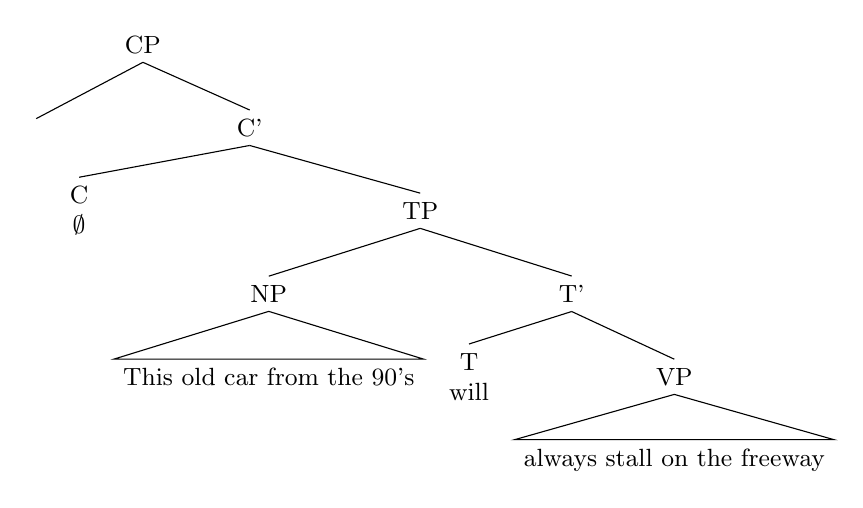
\begin{tikzpicture}
{\small \Tree
[.CP {}
[.C' C\\$\emptyset$ [.TP
	[.NP \edge[roof]; {This old car from the 90's} ]
	[.T' T\\will [.VP \edge[roof]; {always stall on the freeway} ] ]
]%TP
]%C'
]%CP
}
\end{tikzpicture}}\\
The noun phrase is structurally ambiguous between two readings.\\
\noindent\begin{tikzpicture}
{\small \Tree
[.NP D\\This [.N'
	[.AdjP {} [.Adj' Adj\\old {} ] ]
	[.N' [.N' N\\car {} ] [.PP {} [.P' P\\from
		[.NP D\\the [.N' N\\90's. {} ] ]
	]%P'
	]%PP 
	]%N'
]%N'
]
}
\end{tikzpicture}
\noindent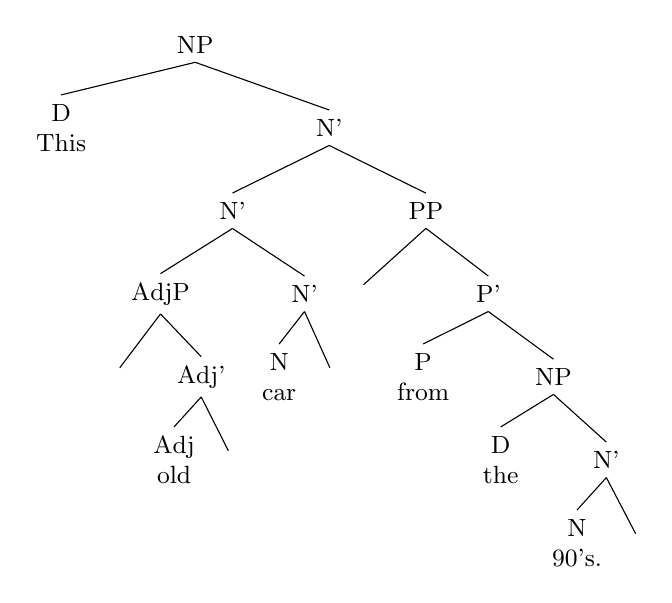
\begin{tikzpicture}
{\small \Tree
[.NP D\\This [.N' [.N'
	[.AdjP {} [.Adj' Adj\\old {} ] ]
	[.N' N\\car {} ]
	]%N'
	[.PP {} [.P' P\\from
		[.NP D\\the [.N' N\\90's. {} ] ]
	]%P'
	]%PP 
]%N'
]
}
\end{tikzpicture}\\
Likewise for the verb phrase, making four overall possible structural readings for the whole sentence.\\
\noindent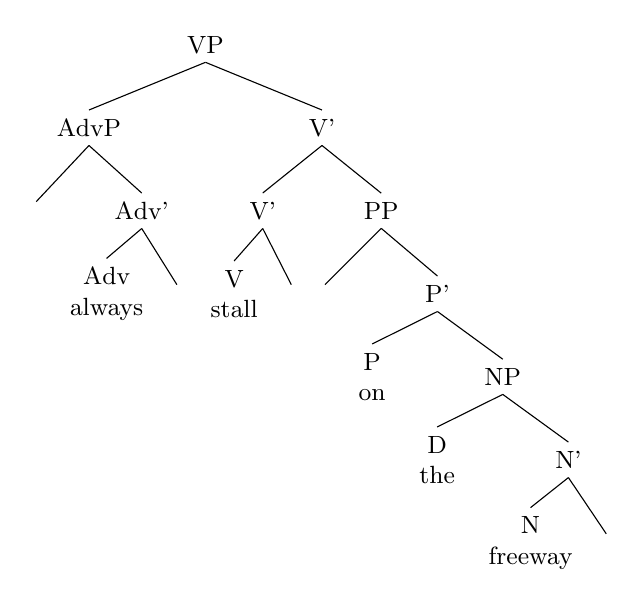
\begin{tikzpicture}
{\small \Tree
[.VP [.AdvP {} [.Adv' Adv\\always {} ] ]
[.V'
	[.V' V\\stall {} ]
	[.PP {} [.P' P\\on
		[.NP D\\the [.N' N\\freeway {} ] ]
	]%P'
	]%PP
]%V'
]%VP
}
\end{tikzpicture}
\noindent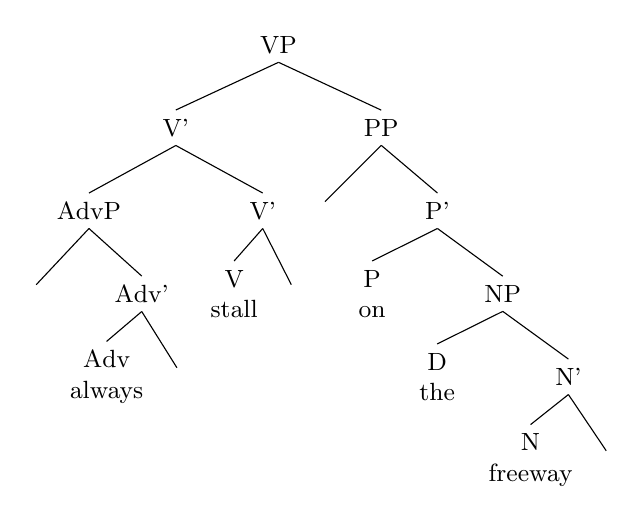
\begin{tikzpicture}
{\small \Tree
[.VP
[.V' 
	[.AdvP {} [.Adv' Adv\\always {} ] ]
	[.V' V\\stall {} ]
]%V'
	[.PP {} [.P' P\\on
		[.NP D\\the [.N' N\\freeway {} ] ]
	]%P'
	]%PP
]%VP
}
\end{tikzpicture}

\item \leavevmode\vadjust{\vspace{-\baselineskip}}\newline
\noindent\resizebox{\textwidth}{!}{\begin{tikzpicture}
{\small \Tree
[.CP C\\$\emptyset$ [.TP
[.NP D\\A [.N' [.AdjP {} [.Adj' Adj\\good {} ] ]
	[.N' N\\language {} ]
]%N'
]%NP
[.T' T\\$\emptyset$
	[.VP [.V' V\\is
	[.NP D\\a [.N' [.N' N\\language {} ]
	[.PP {} [.P' P\\with  [.NP \edge[roof]; {a lot of verbs and a complicated syntax.} ]
	]%NP
	]%N'
	]%PP
	]%NP
	]%V'
	]%VP
]%T'
]%TP
]%CP
}
\end{tikzpicture}}\\

\noindent\begin{tikzpicture}
{\small \Tree
	[.NP
		[.NP D\\a
		[.N' N\\lot
		[.PP {} 
		[.P' P\\of
			[.NP {} 
			[.N' N\\verbs {} ]
			]%NP
		]%P'
		]%PP
		]%N'
		]%NP
		Conj\\and [.NP D\\a
			[.N'
				[.AdjP {} [.Adj' Adj\\complicated {} ] ]
				[.N' N\\syntax {} ]
			]%N'
	    ]%NP
	]%NP
}
\end{tikzpicture}

\item \leavevmode\vadjust{\vspace{-\baselineskip}}\newline
\noindent\resizebox{\textwidth}{!}{\begin{tikzpicture}
{\small \Tree
[.CP {} [.C' C\\$\emptyset$ [.TP
[.NP {} [.N' N\\Tim {} ] ]
[.T' T\\$\emptyset$ [.VP [.AdvP {} [.Adv' {} Adv\\often ] ]
[.V' V\\wonders
	[.CP {} [.C' C\\if
		[.TP [.NP {} [.N' N\\John {} ] ]
		[.T' T\\$\emptyset$ [.VP {} [.V' V\\has 
			[.NP \edge[roof]; {a good...} ]
			]%V'
			]%VP
		]%T'
		]%TP
	]%C'
	]%CP
]%V'
]%VP
]%T'
]%TP
]%C'
]%CP
}
\end{tikzpicture}}

\noindent\resizebox{\textwidth}{!}{\begin{tikzpicture}
{\small \Tree
[.NP D\\a [.N' [.AdjP {} [.Adj' Adj\\good {} ] ]
	[.N' N\\grasp
	[.PP {} [.P' P\\of
		[.NP D\\the [.N' N\\idea
			[.CP {} [.C' C\\that
			[.TP [.NP {} [.N' N\\Sandy {} ] ]
			[.T' T\\$\emptyset$ [.VP \edge[roof]; {stole the...} ]
			]%T'
			]%TP
			]%C'
			]%CP
		]%N'
		]%NP
	]%P'
	]%PP
	]%N'
]%N'
]%NP
}
\end{tikzpicture}}

\noindent\resizebox{\textwidth}{!}{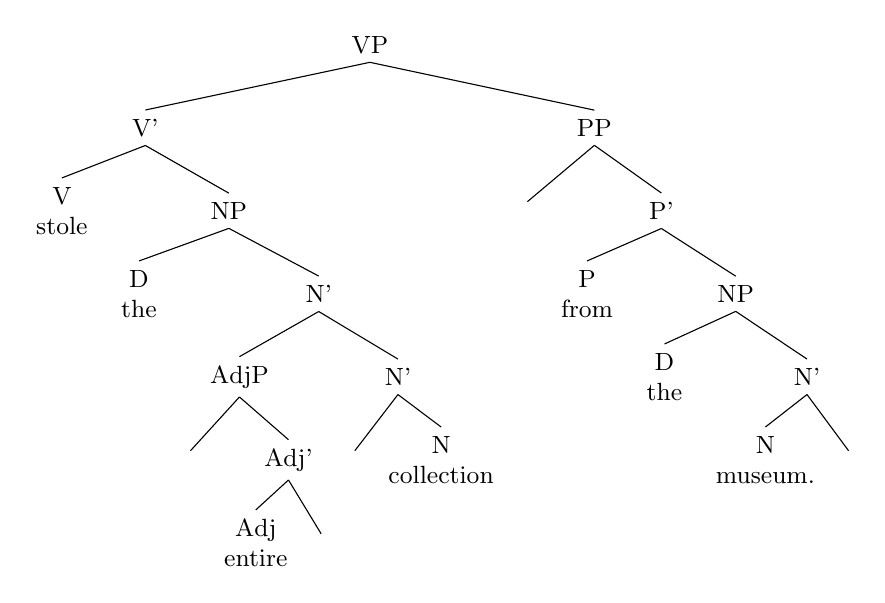
\begin{tikzpicture}
{\small \Tree
[.VP
[.V' V\\stole
	[.NP D\\the [.N' [.AdjP {} [.Adj' Adj\\entire {} ] ]
		[.N' {} N\\collection ]
	]%N'
	]%NP
]%V'
[.PP {} [.P' P\\from [.NP D\\the [.N' N\\museum. {} ] ]
]%P'
]%PP
]%VP
}
\end{tikzpicture}}

\item \leavevmode\vadjust{\vspace{-\baselineskip}}\newline
\noindent\begin{tikzpicture}
{\small \Tree
[.CP {} [.C' C\\$\emptyset$ [.TP
[.NP {} [.N' N\\Syntax {} ] ]
[.T' T\\$\emptyset$ [.VP [.V' {} V\\sucks ] ]
]%T'
]%TP
]%C'
]%CP
}
\end{tikzpicture}

\end{enumerate}

% Question 5
\item Binding Domains\\
\begin{enumerate}[label=\arabic*]
\item Binding Rules
\begin{enumerate}[label=(\Alph*)]
\item An anaphor must be bound in its binding domain.
\item A pronoun must be free in its binding domain.
\item An R-expression must be free.
\end{enumerate}
\item *Michael$_{\emph{i}}$ loves \emph{him$_{i}$}.\\
This sentence violates Principle B. The pronoun \emph{him} is co-indexed with \emph{Michael}. The binding domain for \emph{him} is the main clause, and the noun \emph{Michael} C-commands \emph{him} in this domain, therefore \emph{him} is bound by \emph{Michael}.
\item *He$_{\emph{i}}$ loves \emph{Michael$_{i}$}..\\
This sentence violates Principle C. The R-expression \emph{Michael} is co-indexed with the pronoun \emph{he}. \emph{He} also C-commands \emph{Michael}, therefore the R-expression \emph{Michael} is not free.
\item *Michael's$_{\emph{i}}$ father loves \emph{himself$_{i}$}.\\
This sentence violates Principle A. The anaphor \emph{himself} is co-indexed with the noun \emph{Michael}. However, since \emph{Michael} is dominated by the NP \emph{Michael's father} (of which the head is \emph{father}), it does not C-command \emph{himself}, since the anaphor \emph{himself} is not also dominated by \emph{Michael's father}. Therefore, the anaphor \emph{himself} is not bound within its binding domain.
\item *Michael's father$_{\emph{i}}$ loves \emph{him$_{i}$}.\\
This sentence violates Principle B. The pronoun \emph{him} is coindexed with the noun \emph{father} in its binding domain, which is the main clause. Since \emph{father} is the head of the NP \emph{Michael's father}, \emph{father} C-commands \emph{him}, and thus the pronoun \emph{him} is not free within its binding domain.
\item *Susan$_{\emph{i}}$ thinks that Mary's$_{\emph{j}}$ son should marry \emph{herself$_{i/j}$}.\\
Both readings of this sentence violate Principle A. The anaphor \emph{herself} is coindexed with either \emph{Susan} or \emph{Mary}. \emph{Susan} is outside the anaphor's binding domain, which is the subordinate clause introduced by \emph{that}, therefore it cannot bind \emph{herself}. \emph{Mary} is dominated by the NP \emph{Mary's son}, of which \emph{son} is the head, therefore \emph{Mary} does not C-command \emph{herself}, as \emph{herself} is not dominated by the NP \emph{Mary's son}. Thus, the anaphor is free within its binding domain.
\item John thinks that Susan$_{\emph{i}}$ should kiss \emph{her$_{i}$}.\\
This sentence violates Principle B. The pronoun \emph{her} is co-indexed with the noun \emph{Susan} in its binding domain, which is the subordinate clause introduced by \emph{that}. The NP \emph{Susan} C-commands \emph{her}, therefore the pronoun is not free within its binding domain.
\end{enumerate}
% question 6
\item The binding domain for Japanese is more broadly defined than that of English. As (4c) demonstrates, an anaphor in a subordinate clause can be bound by an NP in the parent clause (i.e. \emph{zibun} can be co-indexed to \emph{Taroga}). Thus, I define the binding domain as follows:
\begin{enumerate}
\item \emph{Binding domain}: The highest CP dominating the NP (anaphor, pronoun or R-expression).
\suspend{enumerate}
Contrast this to English, where an NP's binding domain is only the immediate clause containing it.\\
Sentences (4a,b) demonstrate that a dative NP cannot bind an accusative NP in the same VP. If we assume that both the dative and accusative are complements of the VP (and, thus, are sisters), then we can adjust the definition of binding to account for this behavior.
\resume{enumerate}
\item Principle A: An anaphor must be bound in its binding domain. That is, the anaphor must be C-commanded by an NP that it itself does not C-command.
\suspend{enumerate}
Note that in the English sentence below, \emph{Natsuko} cannot co-index \emph{himself} because \emph{Natsuko} is dominated by a PP and therefore does not C-command \emph{himself}.
\resume{enumerate}
\item Taro$_{\emph{i}}$ showed himself$_{\emph{i/*j}}$ \emph{to Natsuko}$_{\emph{j}}$.
\suspend{enumerate}
Moving \emph{Natsuko} to a complement position allows for it to be co-indexed.
\resume{enumerate}
\item Taro$_{\emph{i}}$ showed \emph{Natsuko}$_{\emph{j}}$ himself$_{\emph{i/j}}$.
\end{enumerate}
This demonstrates the need for a different binding rule in Japanese.
\end{enumerate}

\end{document}
